\documentclass[10pt]{exam}
\usepackage[hon]{template-for-exam}
\usepackage{graphicx}

\title{Potential Difference}
\author{Rohrbach}
\date{\today}

\begin{document}
\maketitle

\begin{questions}
  \question
    Consider a cathode ray tube that is 30 cm long. A potential difference of 35~volts is applied between the cathode and the anode of the tube.

    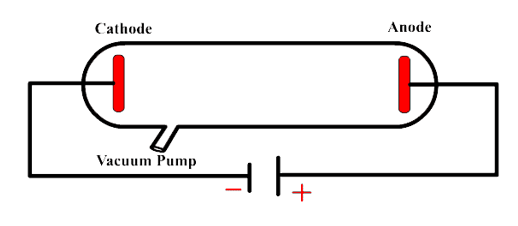
\includegraphics[width=7cm]{CathodeRay.png}

    \begin{parts}
      \part
        Which way would the electron be accelerated through the tube? \vspace{2em}
      \part
        How much work would be done on the electron? \vs
      \part
        Assuming that all the work turns into kinetic energy, how fast would the electron be going when it made it across the entire tube? \vs
    \end{parts}

  \question 
    What is the work done on a $\text{He}^{2+}$ ion that accelerates through a potential difference of $-2.5$~kV. Express your answer in J and in eV. \vs[2]

\pagebreak
  \question
    Use the equipotential lines below to draw an electric field. What kind of charges are these?

    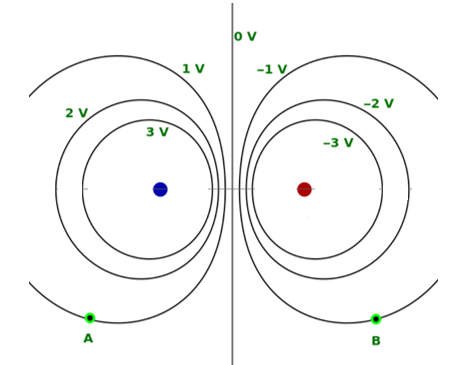
\includegraphics{equipotential.png}


\end{questions}

\end{document}